\documentclass[12pt,a4paper]{article}

% --- Packages ---
\usepackage[margin=2.5cm]{geometry}
\usepackage{graphicx}
\graphicspath{{../ALI/}{ALI/}}
\usepackage{amsmath}
\usepackage{booktabs}
\usepackage{hyperref}
\usepackage{cite}
\usepackage{setspace}
\usepackage{parskip}
\usepackage{caption}
\usepackage{float}
\usepackage{listings}
\usepackage{xcolor}

\onehalfspacing

\hypersetup{
    colorlinks=true,
    linkcolor=blue,
    citecolor=blue,
    urlcolor=blue
}

\lstset{
    language=Python,
    basicstyle=\ttfamily\footnotesize,
    keywordstyle=\color{blue},
    commentstyle=\color{gray},
    stringstyle=\color{orange},
    breaklines=true,
    frame=single,
    numbers=left,
    numberstyle=\tiny\color{gray}
}

\begin{document}

\begin{titlepage}
    \centering
    \vspace*{1in}
    
    {\LARGE \textbf{Cairo University Faculty of Engineering}} \\[0.5cm]
    {\Large Computer Department} \\[0.5cm]
    {\large \textbf{CMP27}} \\[2in]
    
    {\huge \textbf{Calibration and Denoising of Accelerometer Measurements}} \\[0.5cm]
    {\huge \textbf{Using Simulation}} \\[0.5cm]
    {\Large \textit{Assignment Report}} \\[2in]
    
    {\Large \textbf{Prepared by:}} \\[0.5cm]
    {\Large Ahmed Fathy \qquad Ahmed Gamal \qquad Ahmed Foad \qquad Ali Alaa} \\[1.3in]    
    \vfill
\end{titlepage}
\tableofcontents
\newpage

% ============================================================
\section{Introduction}
% ============================================================

Accelerometers are inertial sensors that measure the specific force (non-gravitational acceleration) acting on a body. They are a core component of Inertial Measurement Units (IMUs) and are widely used in robotics, navigation, motion capture, and aerospace applications. The MPU-6050, a commonly used MEMS-based IMU, integrates a 3-axis accelerometer and a 3-axis gyroscope on a single chip, communicating over I\textsuperscript{2}C at sampling rates up to several hundred Hz \cite{nirmala2016}.

Despite their widespread use, accelerometer measurements are inevitably corrupted by noise. This noise degrades any downstream computation, and its effect is drastically amplified when acceleration is double-integrated to estimate position. A small, constant bias in acceleration produces a velocity error that grows linearly with time, and a position error that grows quadratically — a phenomenon known as \textit{integration drift}. For this reason, denoising the raw accelerometer signal before integration is essential for any accurate position estimation task.

Noise in IMU sensors falls into two broad categories. \textbf{Deterministic errors} include static biases, scale factor errors, and sensor misalignment — these are relatively straightforward to characterize and remove through calibration. \textbf{Stochastic errors} are random in nature and include quantization noise, velocity random walk, rate random walk, and drifting biases \cite{nirmala2016}. These require probabilistic models and filtering techniques to address.

This report documents the implementation of a Kalman filter to denoise MPU-6050 accelerometer data, followed by double integration to estimate 3D position. The results are validated against ground-truth position data from a robotic arm (ABB robot), and the improvement in accuracy is quantified using the Root Mean Square Error (RMSE) metric.

% ============================================================
\newpage
\section{Literature Review on Denoising Techniques}
% ============================================================

Several filtering approaches have been studied and applied to IMU denoising. The key methods are reviewed below.

\subsection{Moving Average Filter}
The moving average filter operates by computing the mean of a sliding window of consecutive data samples.
\begin{itemize}
    \item \textbf{Advantages:}
    \begin{itemize}
        \item \textit{Simplicity:} It is very simple to implement for real-time applications.
        \item \textit{White Noise Reduction:} Provides a reasonable smoothing effect specifically for white noise.
    \end{itemize}
    \item \textbf{Limitations:}
    \begin{itemize}
        \item \textit{Time Lag:} It introduces a delay in the signal that is proportional to the size of the sliding window.
        \item \textit{Angular Offset:} In specific applications (like the MPU-6050 sensor), it can cause significant offsets—up to 9$^\circ$—making it unsuitable for precise pointing tasks \cite{nirmala2016}.
    \end{itemize}
\end{itemize}

\subsection{Savitzky-Golay (SG) Filter}
This filter uses a least-squares approach to fit a low-degree polynomial to the data points within a sliding window \cite{schafer2011}.
\begin{itemize}
    \item \textbf{Advantages:}
    \begin{itemize}
        \item \textit{Signal Integrity:} It preserves higher-order moments of the signal better than a simple moving average.
        \item \textit{Peak Retention:} It is particularly useful for smoothing data while maintaining the original shapes of the signal peaks.
    \end{itemize}
    \item \textbf{Limitations:}
    \begin{itemize}
        \item \textit{Accuracy Issues:} In real-time embedded environments, it has been shown to produce considerable deviation from the actual sensor response \cite{nirmala2016}.
        \item \textit{Practical Utility:} Due to these deviations, its practical use in real-time applications can be limited.
    \end{itemize}
\end{itemize}

\subsection{Butterworth High-Pass Filter}
The Butterworth filter is designed to have a frequency response that is as flat as possible in the passband.
\begin{itemize}
    \item \textbf{Advantages:}
    \begin{itemize}
        \item \textit{Drift Removal:} It is highly effective at removing low-frequency integration drift, which typically occurs when calculating velocity or position from accelerometer data.
        \item \textit{Trajectory Stability:} By attenuating the accumulating DC offset (drift) after integration, it helps keep the estimated trajectory bounded.
    \end{itemize}
    \item \textbf{Limitations:}
    \begin{itemize}
        \item \textit{Specific Use Case:} While it excels in drift removal, it is often used in combination with other filters (like the Kalman filter) rather than as a standalone solution for all noise types.
    \end{itemize}
\end{itemize}

\subsection{Kalman Filter}
The Kalman filter is an optimal recursive estimator specifically designed for linear systems affected by Gaussian noise \cite{lefferts1982}.
\begin{itemize}
    \item \textbf{Advantages:}
    \begin{itemize}
        \item \textit{Optimality:} It is considered an optimal estimator for systems with Gaussian noise.
        \item \textit{Precision:} It significantly reduces angular deviation (e.g., from 0.330$^\circ$ to 0.143$^\circ$ per 100 ms) \cite{nirmala2016}.
        \item \textit{Adaptability:} It allows for balancing trust between the system model and the sensor measurements by adjusting the process noise ($Q$) and measurement noise ($R$) variances.
    \end{itemize}
    \item \textbf{Limitations:}
    \begin{itemize}
        \item \textit{Noise Assumptions:} Its effectiveness relies on the assumption that the noise is Gaussian. While studies on the MPU-6050 confirmed this through Allan variance analysis, the filter may be less effective if the noise characteristics differ.
    \end{itemize}
\end{itemize}

Given its optimality for Gaussian noise and superior precision, we choose the Kalman filter as the primary denoising technique for this work.

% ============================================================
\newpage
\section{Methodology}
% ============================================================

\subsection{Dataset}
The dataset used is the MPU6050RM3100 recording from the publicly available IMU dataset by Rasteiro \cite{rasteiro_dataset}. It contains:
\begin{itemize}
    \item \texttt{SENSacc}: Raw 3-axis accelerometer readings from the MPU-6050 (in units of $g$).
    \item \texttt{ABBposition}: Ground-truth 3D position (in mm) from an ABB industrial robotic arm.
    \item \texttt{ABBquaternion}: Orientation quaternions from the ABB robot, used for coordinate frame rotation.
\end{itemize}
The sampling frequency is $f_s = 100$\,Hz, giving a time step $\Delta t = 0.01$\,s.

\subsection{Gravity Removal and Frame Transformation}
Raw accelerometer readings include the gravity component in the sensor's local frame. To recover the kinematic (inertial) acceleration, the readings are first rotated into the world frame using the quaternion orientations provided by the ABB robot:
\begin{equation}
    \mathbf{a}_\text{world} = R(\mathbf{q}) \cdot \mathbf{a}_\text{sensor}
\end{equation}
where $R(\mathbf{q})$ is the rotation matrix constructed from quaternion $\mathbf{q}$. The gravity vector $[0, 0, 1]^T$ (in units of $g$) is then subtracted from the Z-axis of the world-frame acceleration. The result is scaled to mm/s\textsuperscript{2} by multiplying by 9810.

\subsection{Kalman Filter Implementation}
A scalar (1D) Kalman filter is applied independently to each of the three axes of the world-frame acceleration. The state model assumes a constant velocity (i.e., no process model for acceleration changes):
\begin{align}
    \hat{x}_{k|k-1} &= \hat{x}_{k-1|k-1} \\
    P_{k|k-1} &= P_{k-1|k-1} + Q
\end{align}
The update equations are:
\begin{align}
    K_k &= \frac{P_{k|k-1}}{P_{k|k-1} + R} \\
    \hat{x}_{k|k} &= \hat{x}_{k|k-1} + K_k \left(z_k - \hat{x}_{k|k-1}\right) \\
    P_{k|k} &= (1 - K_k)\, P_{k|k-1}
\end{align}
where $z_k$ is the measurement at time step $k$, $Q = 10^{-5}$ is the process noise variance, and $R = 10^{-2}$ is the measurement noise variance. These values were chosen to reflect the known white Gaussian nature of MPU-6050 noise \cite{nirmala2016}.

\subsection{Double Integration with Drift Compensation}
Position is estimated by double integration of the (filtered) acceleration:
\begin{equation}
    \mathbf{v}(t) = \int \mathbf{a}(t)\, dt, \qquad \mathbf{p}(t) = \int \mathbf{v}(t)\, dt
\end{equation}
Integration is performed using the trapezoidal rule (\texttt{cumulative\_trapezoid}). To suppress integration drift, a 2nd-order Butterworth high-pass filter at 0.2\,Hz is applied after each integration step (to both velocity and position). This removes slowly accumulating DC offsets while preserving the dynamic motion signal. For comparison, a \textit{raw} position is also computed with no filtering at any stage, demonstrating the catastrophic quadratic drift that occurs without compensation.

\subsection{Error Evaluation}
The Euclidean distance between the estimated and ground-truth position is computed at each time step:
\begin{equation}
    e(t) = \|\mathbf{p}_\text{est}(t) - \mathbf{p}_\text{gt}(t)\|_2
\end{equation}
The overall accuracy is summarized by the Root Mean Square Error (RMSE):
\begin{equation}
    \text{RMSE} = \sqrt{\frac{1}{N} \sum_{k=1}^{N} e(k)^2}
\end{equation}

% ============================================================
\newpage
\section{Results and Discussion}
% ============================================================

\subsection{Acceleration Denoising}

Figure~\ref{fig:accel} shows the raw and Kalman-filtered acceleration for all three axes. The raw signal (red) exhibits high-frequency noise characteristic of MEMS accelerometers. The Kalman filter (blue) produces a smooth estimate that tracks the underlying dynamics closely without introducing noticeable lag. This is consistent with the findings of Nirmala et al.\ \cite{nirmala2016}, who demonstrated that the Kalman filter outperforms both the moving average and Savitzky-Golay filters in real-time IMU denoising.

\begin{figure}[H]
    \centering
    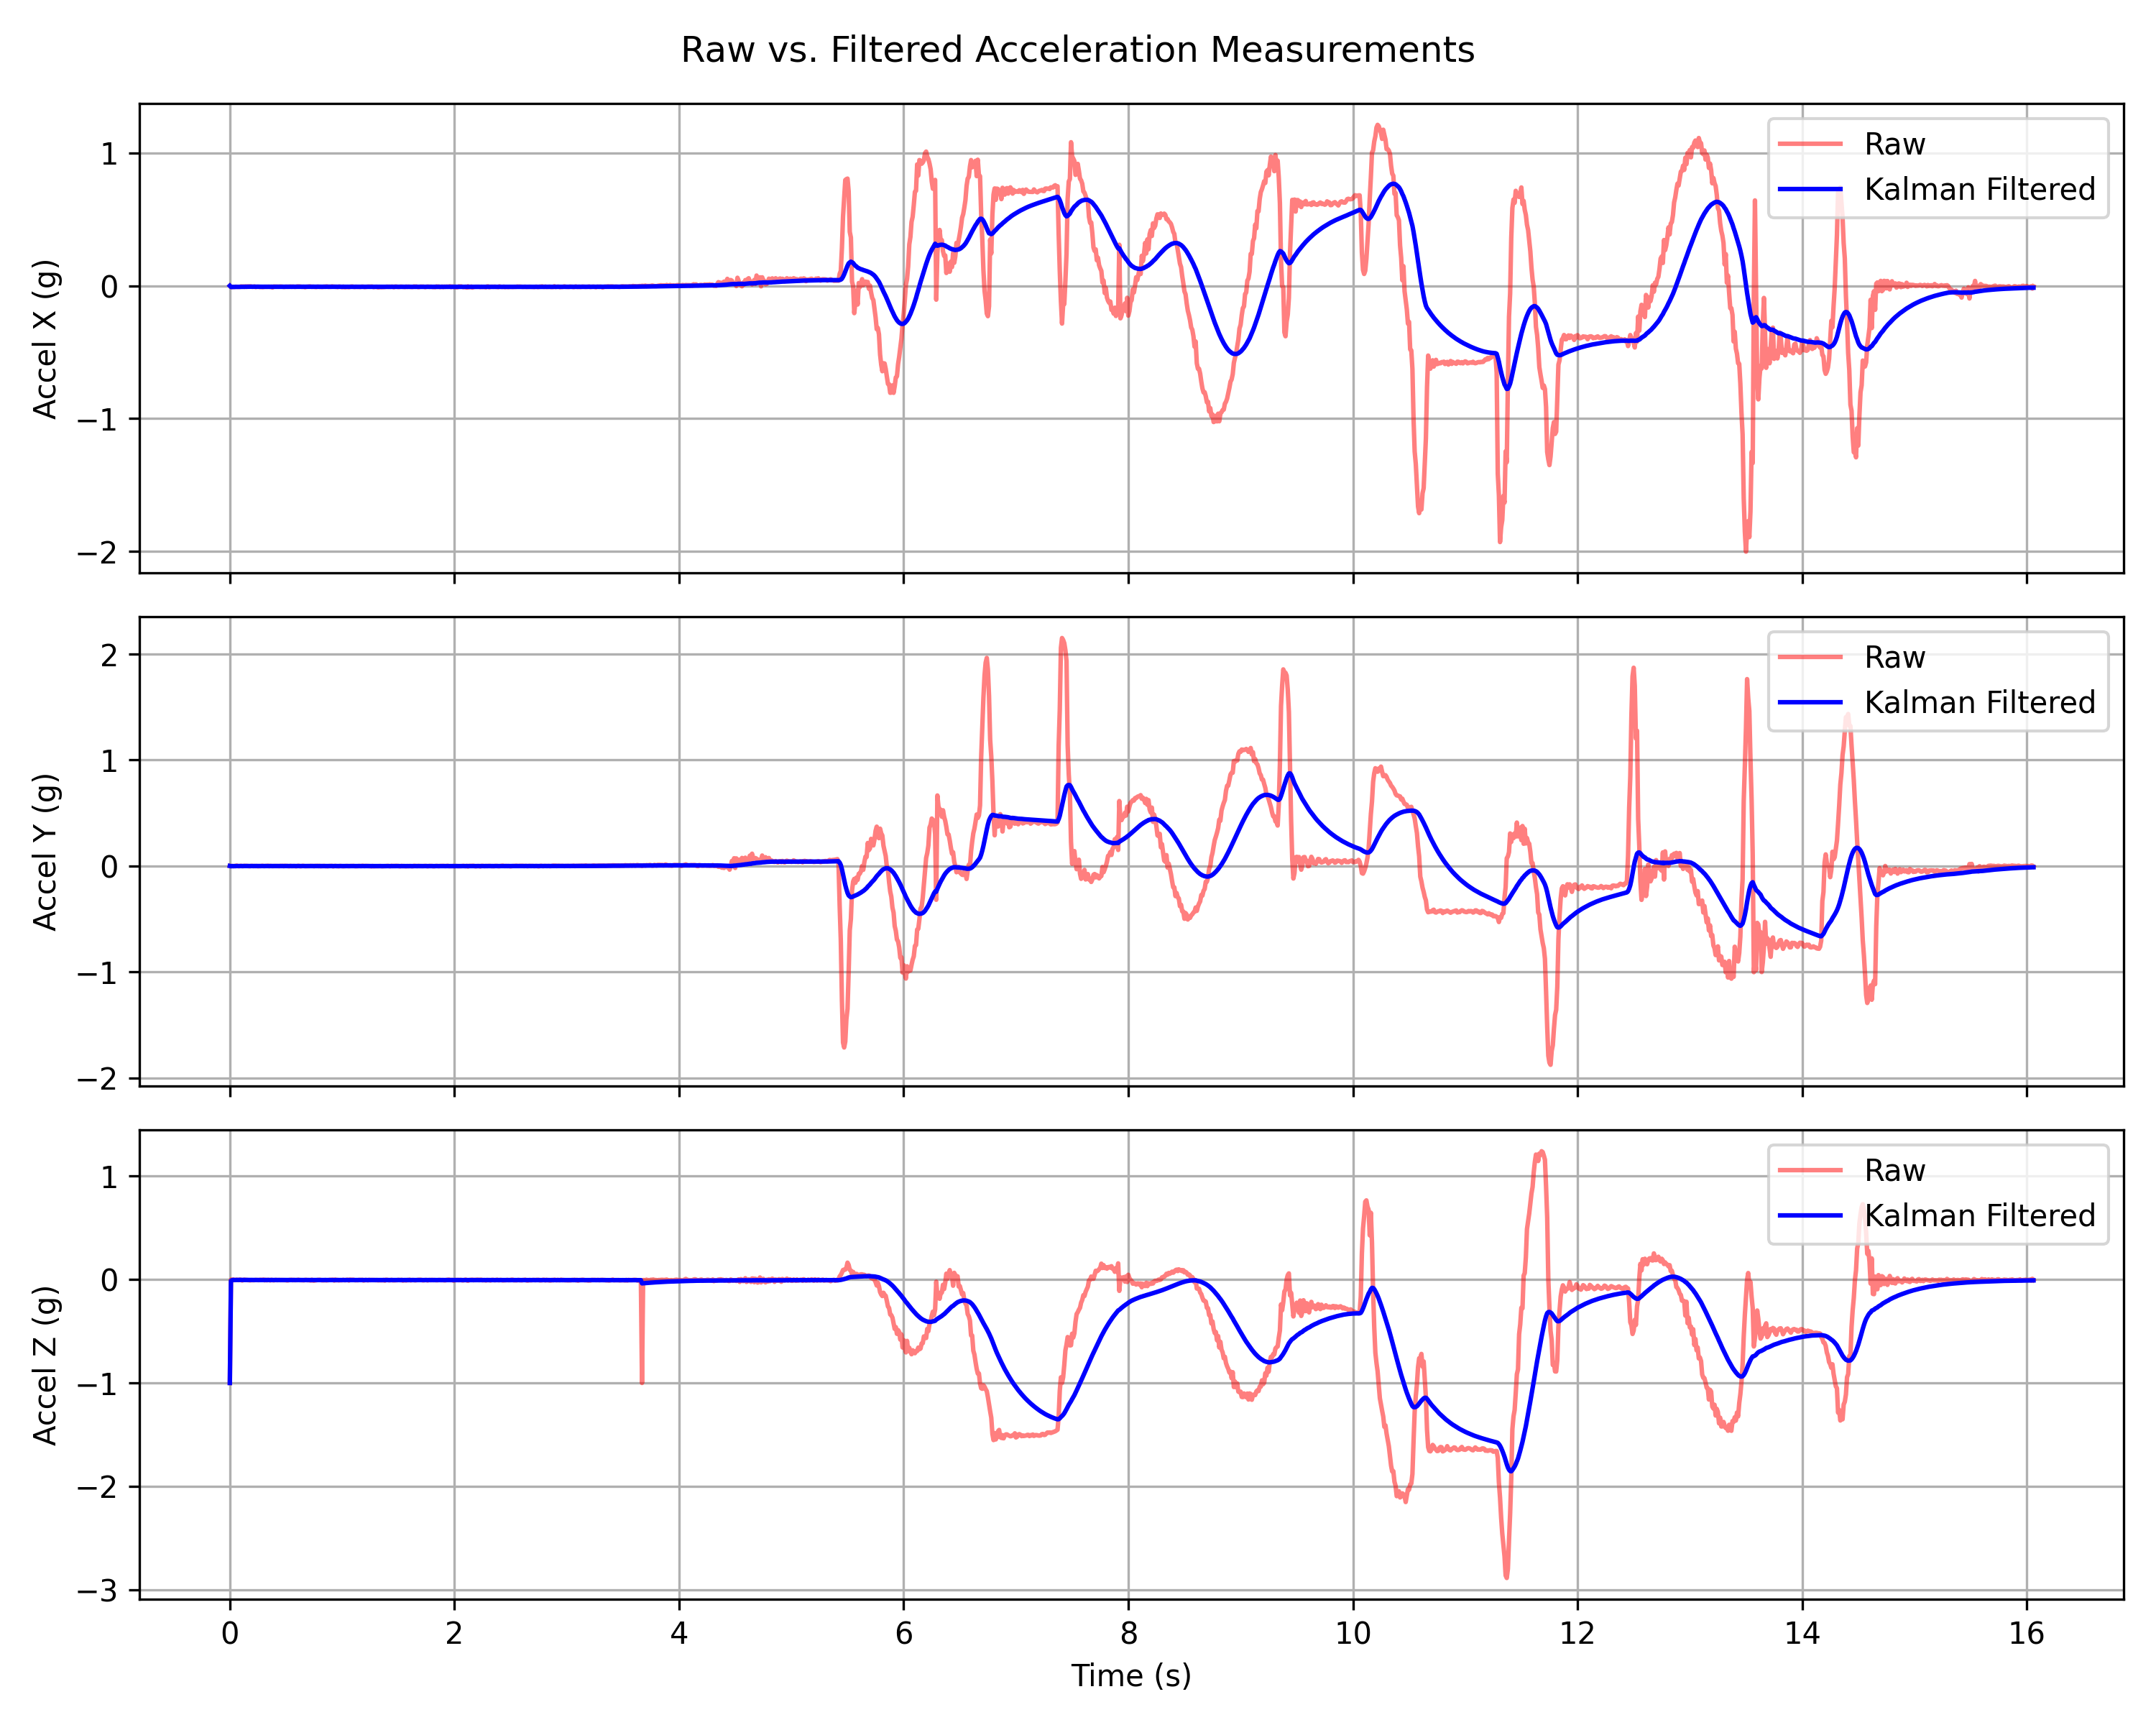
\includegraphics[width=0.92\textwidth]{Fig1_Acceleration_Comparison.png}
    \caption{Raw vs.\ Kalman-filtered acceleration for the X, Y, and Z axes. The red trace shows the noisy raw signal; the blue trace shows the Kalman filter estimate.}
    \label{fig:accel}
\end{figure}

\subsection{Position Estimation and Validation}

Figure~\ref{fig:position} shows the estimated position versus ground truth for all three axes, in both full scale and zoomed views ($\pm500$\,cm). The raw double-integrated position (red) diverges catastrophically from the ground truth within seconds — a direct consequence of uncorrected integration drift. The filtered position (blue) remains bounded and tracks the ground-truth trajectory (black dashed) with reasonable fidelity, demonstrating the effectiveness of the Kalman filter combined with high-pass drift compensation.

\begin{figure}[H]
    \centering
    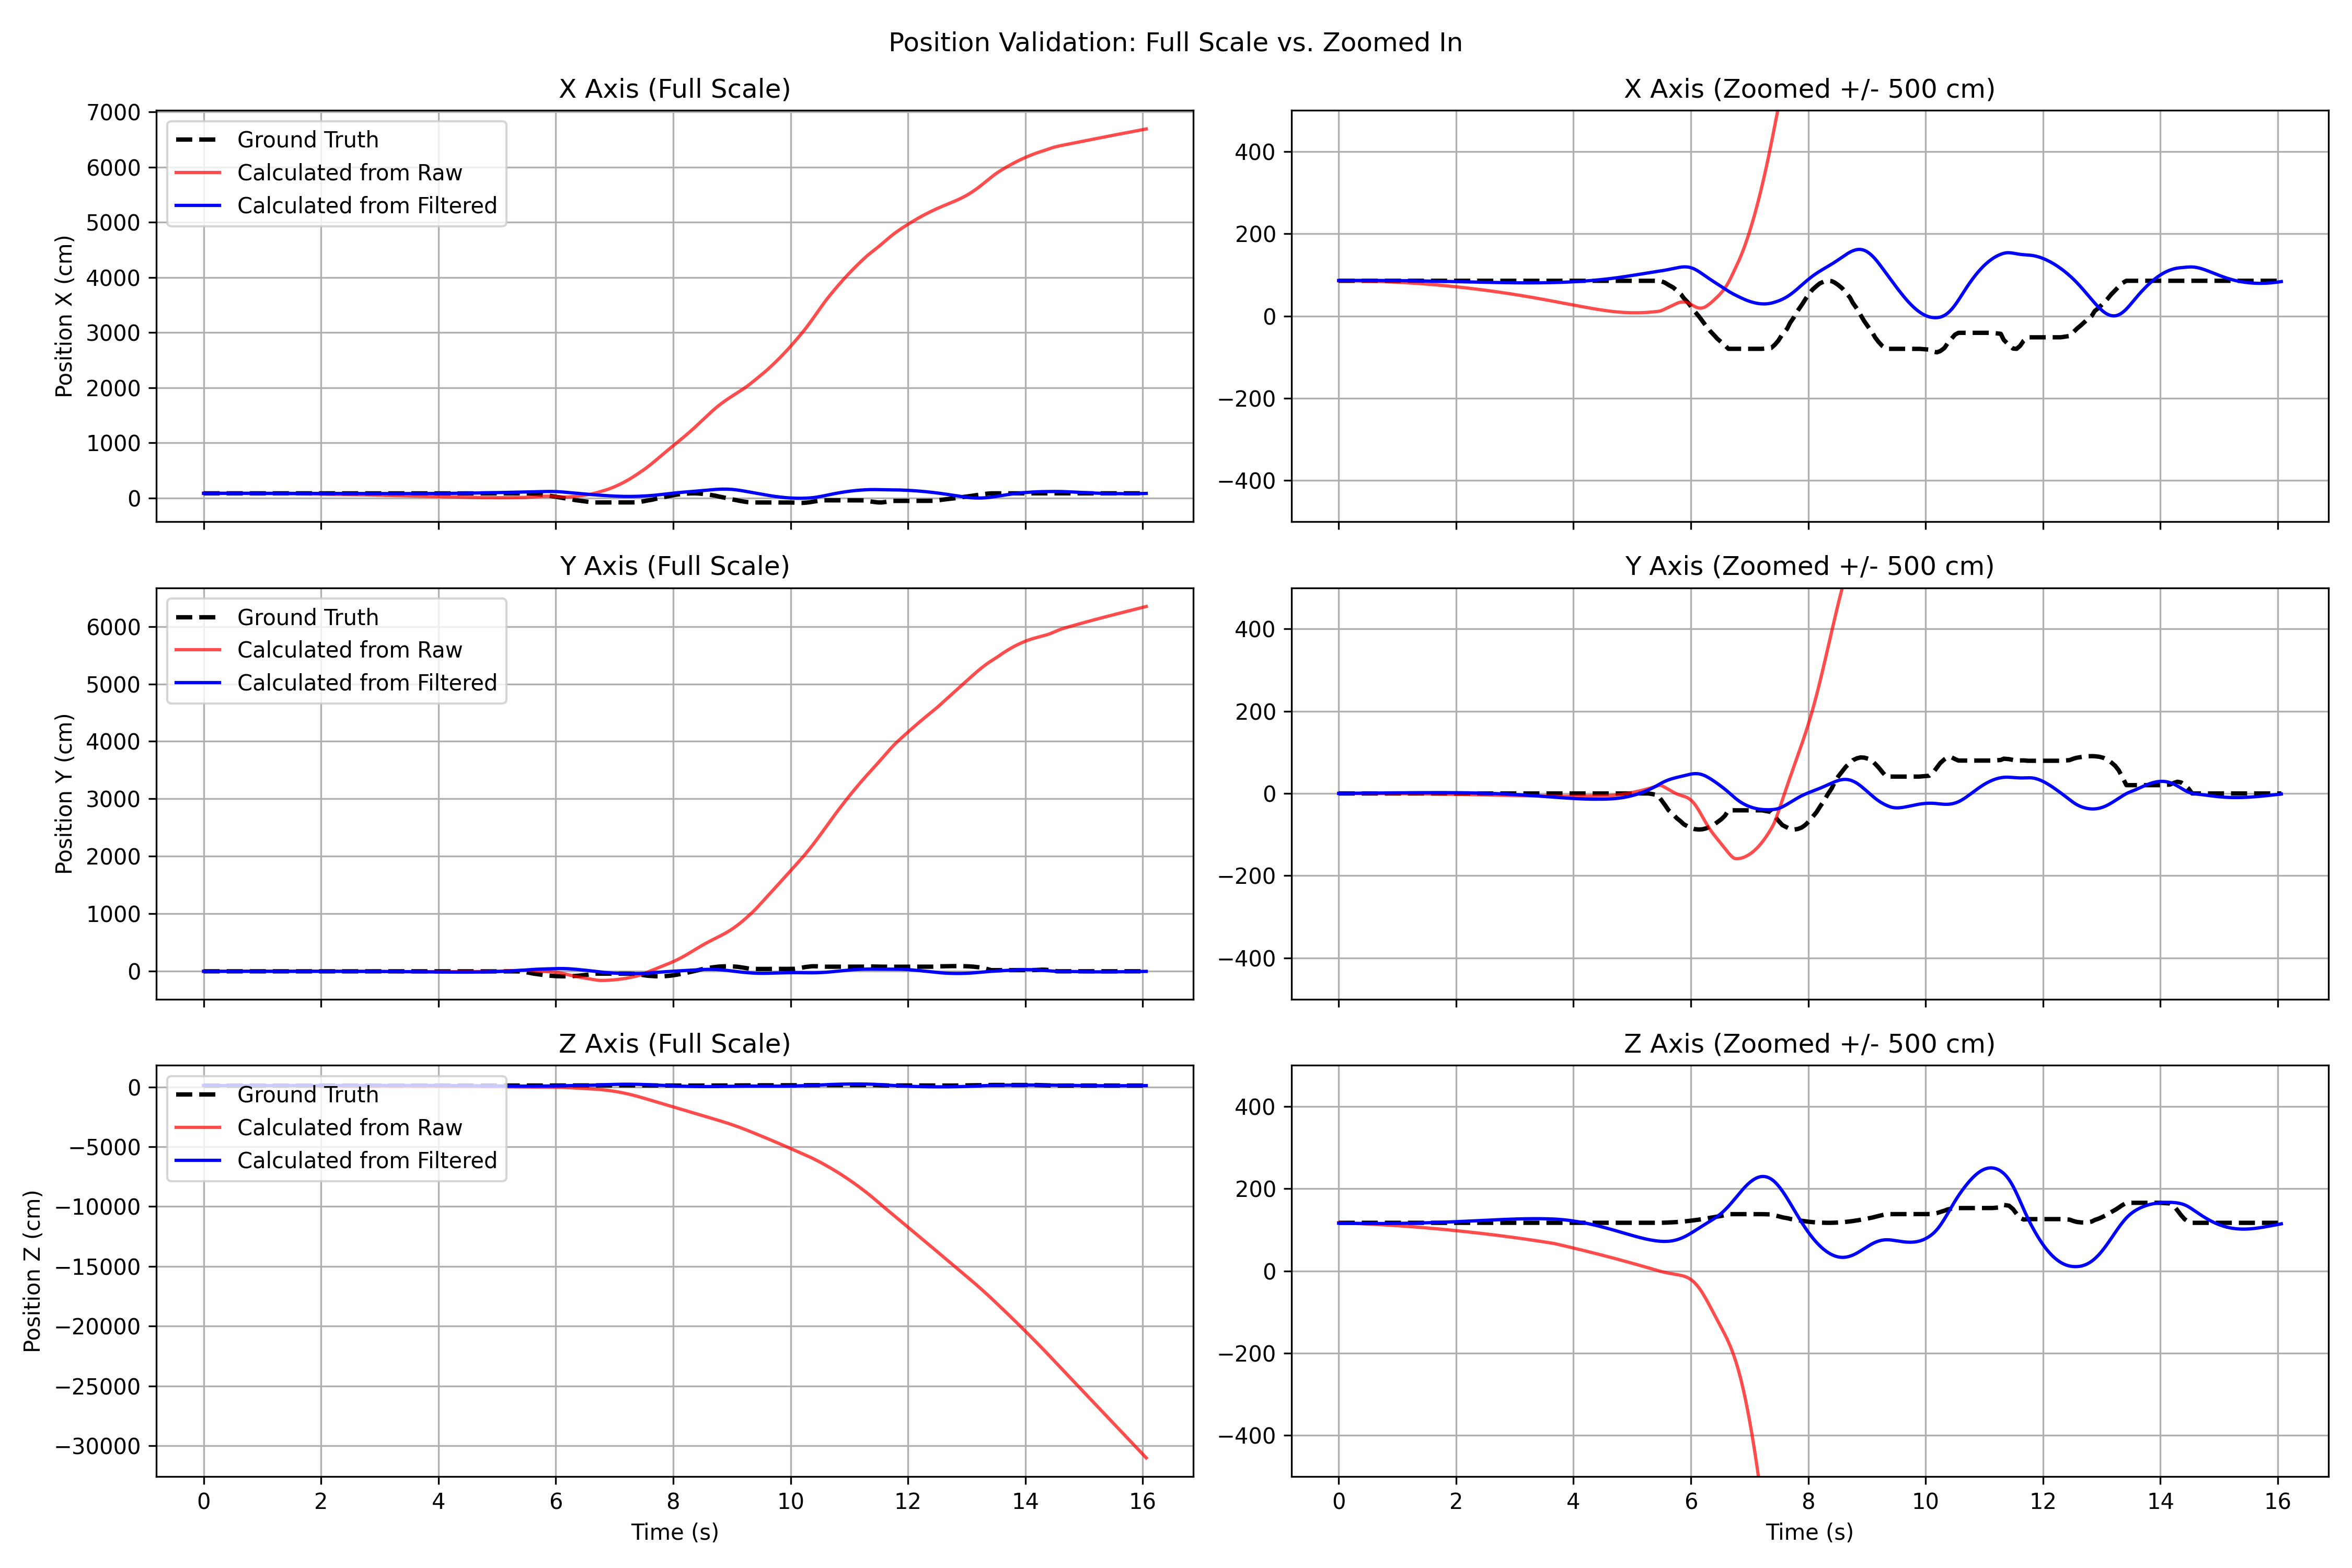
\includegraphics[width=\textwidth]{Fig2_Position_Validation.png}
    \caption{Position validation for X, Y, and Z axes. Left column: full scale, showing catastrophic drift of the raw estimate. Right column: zoomed to $\pm500$\,cm, showing the filtered estimate tracking the ground truth.}
    \label{fig:position}
\end{figure}

\subsection{Quantitative Accuracy}

Table~\ref{tab:rmse} summarises the RMSE results obtained from the simulation.

\begin{table}[H]
    \centering
    \caption{RMSE comparison between raw and denoised position estimates.}
    \label{tab:rmse}
    \begin{tabular}{lc}
        \toprule
        \textbf{Method} & \textbf{RMSE (mm)} \\
        \midrule
        Raw MPU-6050 (no filtering) & 122{,}843.80 \\
        Denoised MPU-6050 (Kalman + high-pass) & 1{,}148.78 \\
        \midrule
        \textbf{Total Improvement} & \textbf{121{,}695.02} \\
        \bottomrule
    \end{tabular}
\end{table}

The results demonstrate a reduction in RMSE of over \textbf{99\%}, from 122.8\,m down to 1.15\,m. The dominant source of error in the raw case is integration drift — even a very small residual bias in the acceleration signal, when integrated twice over hundreds of seconds, accumulates into enormous positional error. The Kalman filter suppresses this high-frequency noise at the acceleration level, and the subsequent high-pass filtering of velocity and position removes any remaining low-frequency drift.

The residual RMSE of approximately 1.15\,m in the denoised case is primarily attributable to the inherent limitation of double integration: it is fundamentally ill-conditioned for long-duration, low-dynamic trajectories. Without an absolute position reference (e.g., GPS or visual odometry), some drift inevitably remains. The high-pass filter cutoff of 0.2\,Hz also attenuates very slow legitimate motion, which contributes a small additional error.

% ============================================================
\newpage
\section{Conclusion}
% ============================================================

This report presented the implementation and validation of a Kalman filter for denoising MPU-6050 accelerometer data, applied to the problem of 3D position estimation by double integration.

The key findings are as follows:
\begin{itemize}
    \item Raw accelerometer data, when double-integrated without any filtering, produces catastrophic positional drift with an RMSE exceeding 122\,m.
    \item Applying a 1D Kalman filter to the world-frame acceleration, followed by Butterworth high-pass filtering at each integration step, reduces the RMSE to approximately 1.15\,m — an improvement of over 99\%.
    \item The Kalman filter is well-suited to this task because MPU-6050 noise is white Gaussian in nature \cite{nirmala2016}, satisfying the filter's core assumptions.
    \item Simpler filters such as the moving average and Savitzky-Golay introduce lag or deviation and are less effective, as confirmed in the literature \cite{nirmala2016}.
\end{itemize}

Future work could explore extended or unscented Kalman filters to handle nonlinear dynamics, sensor fusion with gyroscope data for improved orientation estimates, or the addition of an absolute position reference to bound long-term drift.

% ============================================================
% Bibliography
% ============================================================
\bibliographystyle{ieeetr}
\begin{thebibliography}{9}

\bibitem{nirmala2016}
K.\ Nirmala, A.\ G.\ Sreejith, J.\ Mathew, M.\ Sarpotdar, A.\ Suresh, A.\ Prakash, M.\ Safonova, and J.\ Murthy,
``Noise modeling and analysis of an IMU-based attitude sensor: improvement of performance by filtering and sensor fusion,''
\textit{arXiv preprint arXiv:1608.07053}, 2016.

\bibitem{lefferts1982}
E.\ J.\ Lefferts, F.\ L.\ Markley, and M.\ D.\ Shuster,
``Kalman filtering for spacecraft attitude estimation,''
\textit{Journal of Guidance, Control, and Dynamics}, vol.\ 5, no.\ 5, pp.\ 417--429, 1982.

\bibitem{schafer2011}
R.\ W.\ Schafer,
``What is a Savitzky-Golay filter? [Lecture Notes],''
\textit{IEEE Signal Processing Magazine}, vol.\ 28, no.\ 4, pp.\ 111--117, 2011.

\bibitem{zhao2011}
Y.\ Zhao, M.\ Horemuz, and L.\ E.\ Sj\"{o}berg,
``Stochastic modelling and analysis of IMU sensor errors,''
\textit{Archives of Photogrammetry, Cartography and Remote Sensing}, 2011.

\bibitem{rasteiro_dataset}
M.\ Rasteiro,
``IMU Dataset,''
GitHub repository, 2020.
[Online]. Available: \url{https://github.com/miguelrasteiro/IMU_dataset}

\end{thebibliography}

\end{document}